\documentclass{standalone}
\usepackage{tikz}
\usepackage{ctex}
\setCJKmainfont{Noto Serif CJK SC}
\usepackage{mhchem,siunitx}
\begin{document}
\small
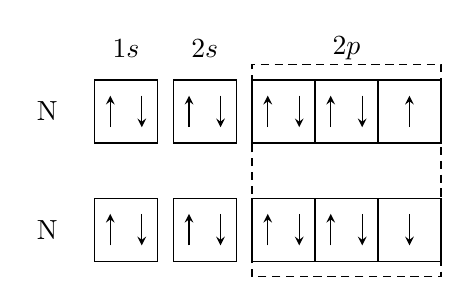
\begin{tikzpicture}[scale=1.0,>=stealth]
  \foreach \x in {0,1,2,2.8}
  {
    \draw(\x,0)rectangle++(0.8,0.8);
    \draw[->](\x+0.2,0.2)--++(0,0.4);
    \draw[->](\x+0.6,0.6)--++(0,-0.4);
    \draw[->](\x+0.2,-1.3)--++(0,0.4);
    \draw[->](\x+0.6,-0.9)--++(0,-0.4);
    \draw(\x,-1.5)rectangle++(0.8,0.8);
  }
  \foreach \x in {3.6}
  {
    \draw(\x,0)rectangle++(0.8,0.8);
    \draw[->](\x+0.4,0.2)--++(0,0.4);
    % \draw[->](\x+0.6,0.6)--++(0,-0.4);
    % \draw[->](\x+0.2,-1.3)--++(0,0.4);
    \draw[->](\x+0.4,-0.9)--++(0,-0.4);
    \draw(\x,-1.5)rectangle++(0.8,0.8);
  }
  \node at (-0.6,-1.1) {\ce{N}};
  \node at (-0.6,0.4) {\ce{N}};
  \foreach \x/\y in {0.4/1s,1.4/2s,3.2/2p}
  {
    \node at (\x,1.2) {$\y$};
  }
  \draw[densely dashed] (2.0,-1.7)rectangle(4.4,1.0);
\end{tikzpicture}
\end{document}